\documentclass{l3proj}

\begin{document}

\title{Developing a chatbot for the University of Glasgow}

\author{Mohammad Alnakhli \\
        James Conway \\
        Samuel Cook \\
        Leonore Papaloizos}

\date{\today}

\maketitle

\begin{abstract}
University staff often receive enquiries that are repetitive, and simple to answer. The process of answering these is nonetheless time-consuming. A long-term student project was undertaken to develop a chatbot for the University of Glasgow to help with this problem. The main focus of this paper is to reflect on our achievements working on this project as a team and on the challenges we encountered during our development process.

\end{abstract}

%% Comment out this line if you do not wish to give consent for your
%% work to be distributed in electronic format.
\educationalconsent

\newpage

%==============================================================================
\section{Introduction}

This paper documents a student team's experience developing a chatbot as a solution to help manage the increasing volume of application and course enquiries which the University of Glasgow's External Relations office receives every year. It details what we did and learned throughout the course of the project.

The paper begins with our \nameref{sec:background} which explains in more detail our customers' motivations for the project and how we aimed to fulfill their requirements. It also summarises our key achievements and quickly reviews what technical challenges were involved.

The two sections that follow reflect on our experiences during the project. The \nameref{sec:rationale} section discusses how the technical challenges we encountered influenced our choice of components and system architecture. \nameref{sec:methodology} then details how we implemented Software Engineering techniques in our development process in order to ensure efficiency, and the challenges we faced along the way.

Finally, our \nameref{sec:conclusion} discuss what we learned as a team from working on this project, and how these lessons can be applied more broadly to help us in developing future projects.

%==============================================================================
\section{Case Study Background}
\label{sec:background}

\subsection{The University of Glasgow's External Relations Directorate}

The University of Glasgow is a well-established academic institution. It is organised into eight directorates, all of which provide different services. External Relations' focus is on course admissions, marketing, student recruitment and mobility, and widening participation at the University. In particular, the `Admissions' and `Short Courses' teams respectively deal with application procedures and policies for undergraduate and postgraduate applicants and students, and providing short course opportunities from the Centre of Open Studies.

\subsection{Motivation}

Chatbot development is a growing field in technology. According to Google Trends, interest in chatbots has quadrupled in the past three years\cite{googletrends}. They are becoming an increasingly popular way of improving and modernising customer service. Chatbots work with natural language to answer customer questions\cite{SLP:Jurafsky}, and as such are not limited like FAQ pages. They are able to respond instantly to queries for multiple users, and are not limited to staff hours\cite{chatbotbenefits}. Example success projects in the world of academia are Whatuni's Luna and ivy.ai's service for universities\cite{educationchatbots}.

Many of the queries the Admissions and Short Courses staff receive are repetitive, but take up significant staff resources to answer. Our project's success would allow staff to respond to these enquiries in a resource efficient way, reducing workload, while also alleviating student concerns by providing quick answers to common questions\cite{educationchatbots}. Staff resources could then be redirected to help students with more detailed cases. A chatbot service would also modernise the University's image and feed into the guidelines of how similar projects could be scaled to other University teams.

\subsection{Project Aims}

With an open-ended project such as a chatbot, we had to make sure to limit our initial requirements to an attainable set. As such, we worked on user stories, which are discussed in more detail in \nameref{subsec:get_reqs}, and decided on the following initial requirements:
\begin{itemize}
\item A user should be able to enter sentences into the system that the chatbot can understand.
\item The chatbot should be able to handle queries relevant to the given datasets and retrieve information relevant to the query.
\item The application should integrate with the University website for easy access.
\item The chatbot should redirect the user to a human when it cannot answer a question.
\end{itemize}

\subsection{Key Achievements}

The main technical challenge for this project was gathering enough knowledge on Natural Language Processing (NLP) to be able to create a dialogue agent. Following research and development, we delivered a functional chatbot, hosted online and accessible to anyone. The application is easily deployable with Docker, which was a challenging process because of the chatbot's CPU-heavy NLP features which had to be containerised accordingly. The chatbot itself can give instant, concurrent, 24/7 responses for a large range of questions, on short courses, postgraduate courses, and common questions, such as the meaning of terminology. We challenged our familiarity with the MySQL database by migrating to Elasticsearch, which allows for much more flexible and scalable data storage. We designed an appealing chat interface, with a design conforming to the University marketing guidelines\cite{brandguidelines}. Conversation is guided through both free user input and buttons to maintain the dialogue's context, and the chatbot is able to redirect the user to an appropriate member of staff if necessary. We also implemented a chat logging system for staff to monitor the performance of the bot and gather information to better understand the needs of users. Additionally, we only used open-source libraries and frameworks to develop our chatbot, rather than popular commercial solutions, meaning that our customers would not depend on a commercial product in order to run our application.

%==============================================================================

\section{Research and Development}
\label{sec:rationale}

\subsection{Approaching Natural Language Processing}

There were a large number of available NLP frameworks for our project, all of which we were inexperienced with. The main factors we considered for our choice of framework were its ability to couple with other project components (database, chat interface), its overall features (dialogue engine, accurate intent and entity classification), and its ease of use for developers. We eventually narrowed our choices down to Google's Dialogflow and the open-source Rasa Stack.

We worked on prototype applications using each option to gain a good grasp of their functionality. There was a trade-off made between this additional effort and reducing the risk of making a wrong choice early on. We found that Dialogflow's strongest feature was its intuitive UI. Despite this, we concluded that Rasa was more suitable. A Rasa agent has to be built using Python, which makes it more flexible than Dialogflow's closed source code. Rasa's data is also hosted locally, as opposed to Dialogflow's cloud hosting, meaning our clients could have full control over the chatbot's data. Lastly, choosing open-source meant there was no need to worry about organising a subscription with the customer for the service or how its features could be limited by the amount that was paid for it. Rasa's open-source feature also proved to be very useful at a couple of instances when team members found themselves at an impasse, unable to debug their code. As highlighted in ``The Cathedral and the Bazaar", open-source projects have the benefit of having a community of developers to help with debugging, which increases the chance that a problem would be ``transparent to somebody" who could help\cite{cathedral:Raymond}. We were able to open issues on Rasa's Github repository to try and get another helping hand on debugging from Rasa developers, who helped us fix bugs that had been hindering our progress.

\subsection{From the University Data to the Database}

The customers provided us with sample course datasets so that the chatbot could return relevant data during development. Both the short courses and the postgraduate courses data were provided as Excel sheets. Our first approach to storing this data for querying was to use a MySQL database, as we were all familiar with it. However, we faced problems such as having to find workarounds for missing or duplicate data. Moreover, a lot of the data was very dense and as such, harder for us to query and parse in one step with MySQL. We were able to store all the provided data with MySQL, but we felt that our solution was not the most sustainable or scalable.

Our project supervisor suggested that we migrate to a search and indexing based database, such as Elasticsearch, as we would be able to perform both retrieval by key and by free text search. Switching to Elasticsearch proved to be one of the most beneficial decisions we made during our project. It made working with the data, as well as extending the database much easier. Elasticsearch allowed us to simply add new data through dictionary structures, and had useful query functionality with parameters such as `scoring' or `uncommon words'. Moreover, if needed, the aforementioned dense fields of the provided datasets could be retrieved by content search with Elasticsearch's integrated functionality\cite{elasticsearch}.

Although we had to throw away the MySQL component of our system, we had been aware that this could possibly happen. As F. Brooks writes in the influential work ``the Mythical Man Month",  ``Plan to throw one away: you will, anyhow"\cite{manmonth:Brooks}. The positive impact this migration had on our project and its scalability counterbalanced the daunting task of having to face a new learning curve.

\subsection{Modular System and Integration}

\begin{figure}[h!]
    \centering
    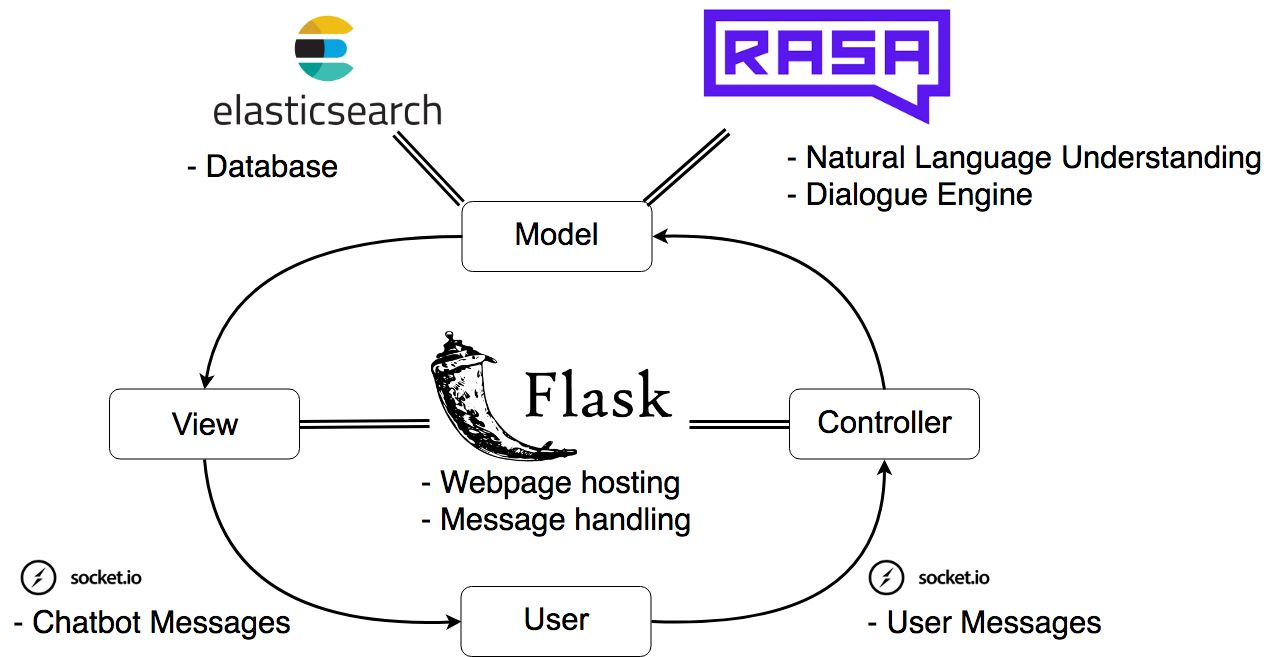
\includegraphics[width=0.75\linewidth]{figures/MVC.jpg}
    \caption{System diagram for our application}
    \label{fig:mvc}
\end{figure}

To make the system modular and easy to integrate, we designed it around the Model-View-Controller pattern as it has the major benefit of achieving the separation of presentation from model\cite{patterns:Fowler}. This splits the concerns of the essential functional parts of the chatbot; the database and conversational A.I., from those of the less important website related parts such as the chat interface as shown in Figure \ref{fig:mvc}. This way, the customer could discard the presentation components if they did not need them, and still have a functional chatbot component which they could then more easily implement into their own presentation system.

In the last week of the project before the code freeze, our clients organised a meeting between us and the University web team who would potentially continue our work after the handover. In the meeting, we discovered that the University website used different technologies to our project. It was too late to adapt our own work to conform with the technologies the University server used, so we agreed with the web team to write comprehensive documentation to make sure they understood the system and its components, and then leave the task of actual integration to them. We learnt that in the future, if working on a similar project which eventually required integration, learning what technologies the end system uses would be a necessary first step.


%==============================================================================

\section{Development Methodology and Agile Practices}
\label{sec:methodology}

\subsection{Team Organisation}

At the start of the project, we assigned the roles of Project Manager, Chief Architect, Secretary, Customer Liaison, Quality Assurer, Testing Manager, Librarian, and Tool Smith to team members. Assigning some of these turned out to be quite useful, particularly Customer Liaison and Secretary, which is discussed in \nameref{subsec:customer_com} and \nameref{subsec:change_mgmt}, respectively. The team struggled more with the details of some of the other roles, which may have benefited the project more had we established clearly what tasks each role-bearer should conduct.

The team split themselves according to an area of development: server and interface, testing, deployment, and NLP. These became our main team roles for the duration of the project. Some team members chose to focus on these areas early on as they believed they were best suited to them, while others who did not have a preference worked more generally on various areas, then as the project progressed they eventually specialised on what they had became more knowledgeable on. For each area, the team member in charge was the first point of contact for any questions or merge requests related to the issue. This allowed everyone to get some sense of leadership and responsibility. Each member had the responsibility to communicate to others of any developments or roadblocks in their side of the project in a ``partnering approach"\cite{leadership:Farley}. We hoped each team member would feel empowered through this setup, although in the future having a clearly designated coordinator might prove beneficial as an authoritative voice to guide tougher decisions when the project calls for it.

\subsection{Team Communication}
The team agreed to communicate through Discord, which allowed us to easily message about different topics through specialised channels. One of the principles guiding Agile development is that “the most efficient and effective method of conveying information to and within a development team is face-to-face conversation”\cite{agilemanifesto}. We wanted to make sure we met at least once every week to review our progress and code in the same environment, so that any questions could be asked and answered immediately.

Still, our first few retrospectives highlighted that we all felt that we struggled with team communication and sharing progress and opinions. To combat this issue, we decided to implement smaller retrospective-like reports on a separate Discord channel on Monday and Friday evenings, where each team member listed what they had been working on in the past few days and reported on their achievements and any problems they had encountered. Subsequent retrospectives highlighted that this massively improved our team communication as well as our understanding of where the project currently stood in terms of functionality.

From this experience, we feel that although we recovered from this flaw, in any future project it would be important for us to communicate our efforts more regularly. If any team member works too independently, actions should be taken more quickly to make sure it does not spiral and affect the project negatively.

\subsection{Customer Communication}
\label{subsec:customer_com}

We met with the clients at least once at the end of every milestone in order to discuss progress as well as receive feedback to identify and prioritise requirements. We also regularly stayed in touch via email to discuss any questions, share relevant data and inform them on our progress.

As we had a client group of five who were all from a non-technical background, it was important for us to make sure to present information in a way which was not heavy on technical language. After the initial customer meeting, we began presenting a live demonstration of our product to our client, in order to showcase new features or developments. The demonstrations took the form of design wireframes in earlier demonstrations[\ref{apdx:wireframes}], and walkthroughs of chat conversations later on. This made sure the customers were made aware of our progress in a form which they understood.

One team member habitually found themselves managing client correspondence and leading email discussions and became our Customer Liaison. This created an issue when another team member attempted to organise an intermittent meeting via email and found that the client failed to respond within the usual timeframe, because they had only been expecting correspondence from the Customer Liaison. This led us to make sure we considered our team roles when assigning tasks to each team member, as well as following up if the client was found to be silent for an unexpected amount of time.

\subsection{Requirements Gathering}
\label{subsec:get_reqs}

At the start of the project, we used ethnographic methods to develop user stories and the adjacent user scenarios to help us define the functionality we wanted to implement. The customers' non-technical background meant that writing user stories  helped us transform their ideas into a set of actionable functional and non-functional requirements at different levels of specificity\cite{userstories:mgs}. To help prioritise our requirements, we separated our user stories into MoSCoW categories. Examples can be found in Appendix \ref{apdx:moscow}.

Requirements gathering is a continuous progress, and as the project developed, the customers would voice suggestions or new requirements they had. One new requirement was to have an admin interface to facilitate the configuration and addition of new data. Although it was decided not to prioritise it due to time constraints, we made sure that our database stayed scalable for new data. Also, before the last iteration, it was suggested that we incorporate a button feature into our chatbot. Despite the late request, in line with the second principle behind the Agile Manifesto, ``Welcome changing requirements, even late in development"\cite{agilemanifesto}, we worked hard in order to implement this feature, undeterred by having to rework a lot of the chatbot's functionality. Occurrences like this ensured that our clients held us in high esteem.

Good developer-client communication ensured that both parties had a uniform understanding of the goals and the prospective outcomes of the project. Although we communicated effectively with our customers on our priorities for each iteration, we failed to clearly formalise our functional and non-functional requirements to them. Thankfully, this did not cause confusion or create any problems between the customers and the development team. We made sure to correct this from milestone five onwards. We became more assertive when discussing requirements, as well as making sure to communicate clearly so as to minimise misinterpretation and ensure that both parties had a good grasp on what progress was to be expected.

\subsection{Project Planning with Issues}

Following a workshop on project planning that highlighted that our task management was inadequate, a conscious effort was made to improve the way issues were stored on our change management system; GitLab. Each team member was to enter issues based on the following guidelines:

\begin{itemize}
\item The aim of the issue should be understandable from the issue title.
\item The issue should be properly labelled with one or more labels.
\item The issue description should elaborate on implementation.
\item The issue's assignee should aim to attach due dates and track progress.
\end{itemize}

\begin{figure}[h!]
    \centering
    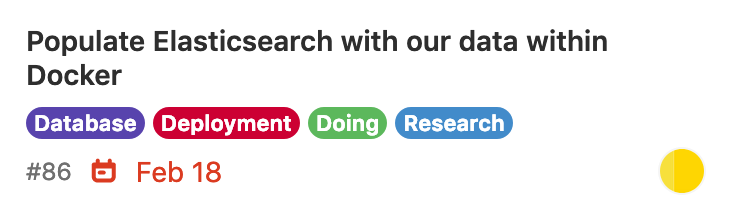
\includegraphics[width=0.4\linewidth]{figures/Project_Planning.png}
    \caption{Example of an issue header from our GitLab}
\end{figure}

Issue numbers should also be referenced in branch names and commit messages. The Secretary took on the role of making sure issues followed these guidelines to facilitate common understanding and organised development.

The importance of storing such artifacts was highlighted when the servers that stored our repository were taken down for security reasons during iteration four. Although the code was moved over to a new repository, team members were finding it hard to make progress as past issues and the Wiki could not be accessed. Some team members made substantial progress, such as completing a database migration, yet did not know how to best reference the closed issue or whether new issues should be made on the new repository.

\subsection{Change Management}
\label{subsec:change_mgmt}

Initially, we used different branches for the different areas of our project, such as NLP or design, in order to avoid pushing unreviewed code directly to the master branch. This was successful until developers began working on related issues and encountered more code conflicts. We then set out to assign one issue per branch. This helped not only to reduce merge conflicts, but also to keep branches from getting too outdated as a result of changes to the master branch. There were particular instances of branches being weeks behind on commits, and then upon requesting a merge request, merge conflicts were so large that merges had to be done locally. To prevent any further issues arising from prolonged and local branches, it was decided that branches had to be reviewed more often for staleness. Reducing the scope that each branch would undertake and pulling from master more often helped prevent these instances of complex code conflicts from reoccurring.

When committing to a branch, we did not always remember to write detailed commit messages, but towards the end of our process, encouraging these practices helped when team members were working on the same branch, and minimised the miscommunications involved when switching branches.

\subsection{Pair Programming}

During our fourth iteration, we held a workshop to try pair programming, during which we separated into pairs and worked to close an issue, swapping roles every 5-10 minutes. This did not prove particularly successful, mainly because the timescale meant that we had little time to get into a proper workflow before having to switch roles. This was worsened by the fact that each team member had specialised in different areas, and was thus more confident and skilled in certain areas than others.

Despite this, it did highlight areas for us to improve upon regarding our team work. After conducting more in-depth code reviews to improve our understanding of one another's code, as well as having multiple people on the team work on NLP, we did attempt pair programming again, with significantly better results. We removed the strict time limit for turnovers, and were better at spotting errors in code. As outlined as a benefit in A. Cockburn and L. Williams' paper ``The Cost and Benefits of Pair Programming", we were able to significantly improve team dynamics as well as give coders a broader understanding of each piece of the system\cite{pairprog}.

\subsection{Quality Assurance}

\subsubsection{Continuous Integration}
\label{subsubsec:ci}

All our commits were checked into a Continuous Integration (CI) pipeline, which ran our test suite as well as built our different components. Our technology stack featured CPU-heavy packages, so checking that the application was still deployable after any changes to the code was a form of quality check. Our CI setup involved containerising our application with Docker. Although a challenging process, it turned out to be an asset for deployment and handover, because it meant that the whole system could be spun up in one command on any system.

\subsubsection{Testing}

%% Unit Testing
It was important for us to have a test suite that checked that the core functionality of our system would not break when adding new features. The Rasa library made it straightforward to extend functionality, but we found ourselves making basic syntax or logic errors which were easily fixed, but meant that we had to restart the chatbot again, which was time consuming. We implemented functions to test the main and elastic Python modules specifically as they played a crucial role in functionality. The implemented unit tests for the main components in the project covered over 90\% of smaller modules. Example of coverage is detailed in Appendix \ref{apdx:coverage}. However, as we were new to the Rasa library, we were unsure of how to test their provided packages. As such, we did not prioritise the testing of our Rasa modules. Reflecting on this, it might have been a big oversight for appropriate quality assurance, and we would prioritise this should we do it again.

%% Behaviour-Driven Development
Early in the project, the Testing Manager also decided to use Behaviour-Driven Development (BDD) to test our application. The decision was made based on the fact that our set of requirements was based on user stories, which BDD is most adapted for\cite{bdd:Goulart}. It would also allow us to test that the chatbot responded correctly to different user inputs, and as such, test correct functionality from the Rasa modules.

\begin{figure}[h!]
  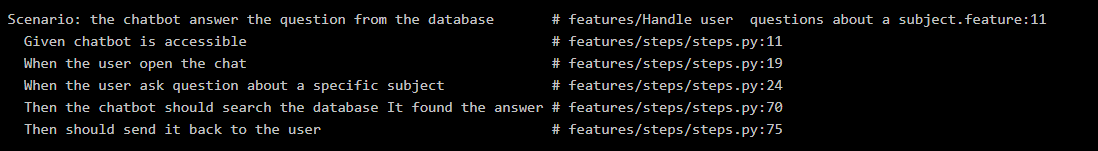
\includegraphics[width=\linewidth]{figures/BDD.PNG}
  \caption{Example of a scenario tested with BDD}
\end{figure}

Unfortunately, we were unable to implement automatic behaviour testing on a local version of our system running on an OpenStack Virtual Machine. Its CPU settings did not allow for Tensorflow support. Issues with the department servers being down and the extended inaccessibility of the OpenStack admin page meant that the team was unable to try and change the settings or research how to bypass the issue within a reasonable timeframe. Therefore, the Testing Manager decided to test the online deployed version. This was not ideal as usually it was not up to date, or the BDD scenarios had not been updated to the latest features due to coding difficulties. In those cases, the tests would fail, and time would be lost trying to understand where the error came from, when the issue was a lack of correlation. This became especially prominent in the last iteration when buttons were implemented to control dialog flow where BDD tests had to be rewritten. Although we felt behaviour-driven development was a good testing practice, we would have liked to implement it more thoroughly.

%% Test-Driven Development
Towards the end of the project, it was felt that the team had relied too much on the Testing Manager to implement the majority of the tests, and we decided to do some test-driven development (TDD) for the last iteration while the code was being refactored and cleaned. Research on TDD found that it improves quality of code, passing 18\% more of black box tests\cite{tdd:George}. Test-driven development allowed us to make sure refactoring and cleaning code was not breaking any previous functionality, and that we were simply making our code easier to use and understand for the future. This ended up being very useful, and revealed that TDD was something we should have been taken more care to implement during earlier stages of the project. On reflection, we feel that it is an essential practice that can benefit any coder.


\subsubsection{Code Reviews}
We required code reviews to be performed before any branch was merged to master. They proved to be essential to our quality assurance. The team hoped that an extra person working to check over the other team member’s code for any errors would help substantiate Linus's law that ``Given enough eyeballs, all bugs are shallow"\cite{cathedral:Raymond}. Code reviews ended up having an extensive positive effect on our team and code quality. It made it easier to spot bugs, and pushed team members to write better code. Google performed a case study on their code review practices, and used those specific reasons as a justification for them\cite{codereview:Google}. Finally, it also meant other team members got the opportunity to gain a better understanding of other team members' work by asking questions on the merge requests and obtaining explanations from the author. This additional positive impact was also highlighted in Google's case study, where they found questions over time lower as developers acquire experience with the codebase\cite{codereview:Google}. Overall, it improved team communication and this was mentioned in the retrospective after the iteration where code reviews were started.

\subsection{Process Improvement with Retrospectives}

We held a retrospective after each customer day to discuss our performance and give critical feedback in order to refine the efficiency of our development process\cite{agilemanifesto}.

We used the 4Ls approach, meaning that we discussed what we liked, lacked, longed for and learned. This helped us take a step back and look at the broader picture to make informed decisions for the next iteration. We observed recurring themes in the `lacked' section of our 4Ls, like ``Better Communication". This was partially down to trying different methods each iteration to try and combat the problem, which proved harder than initially expected. This was refined by putting more focus on the different actions to take, rather than simply identifying the problem.

\begin{figure}[h!]
    \centering
    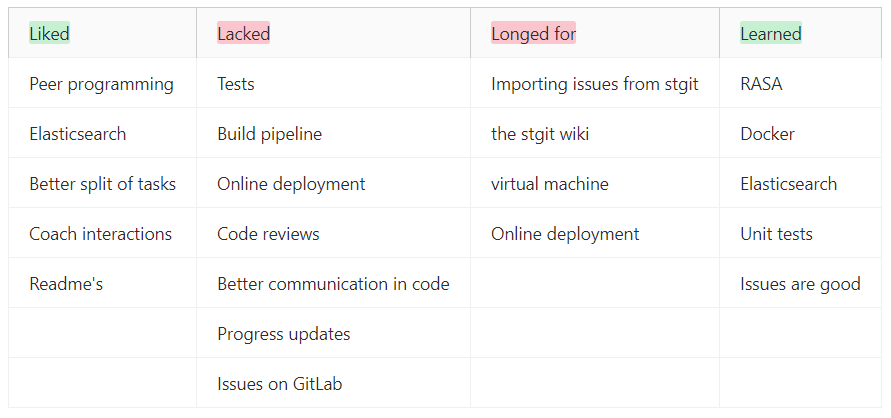
\includegraphics[width=0.85\linewidth]{figures/Process_Improvement.png}
    \caption{4Ls reflection after our fourth iteration}
\end{figure}

After looking at the positives and negatives of our process, we decided on a list of actions to take to improve, as well as a set of objectives. We discussed the lists from the previous iteration and evaluated how well we fulfilled our previous goals, which highlighted what previously assigned actions should be continued.

We then clarified all the issues for the next iteration and held a Planning Poker session in order to estimate the time we would require to complete each one. Our estimates were usually off, because we often had new issues appear after we started the iteration, which would go on to affect the subsequent issues and our estimates. This could be reworked with better issue planning. We also recorded each team member's estimates, as well as the average and the standard deviation values to highlight how much we differed from our original estimate after discussion. Appendix \ref{apdx:pp} shows all our Planning Poker estimates for the last iteration. In the future we could try an alternative approach, such as affinity grouping\cite{agileestimationtechniques:Sliger}, to see if it could provide better estimates.

Overall, we found the retrospectives very helpful. They provided an opportunity for us to make changes in our process, as well as to evaluate our achievements. This was beneficial because it helped us in both scoping and laying out our plans for the next iteration, as well as guided us on avoiding previous mistakes.

\subsection{User Study}

After our work in the fifth iteration allowed us to deploy our chatbot online, it encouraged us to show our latest chatbot prototype to friends and colleagues to get their opinion on its functionality. This provided us with good insight, as they had no prior knowledge of how the system worked. Their feedback justified the rationale that using buttons in the right places to guide the conversation would reduce user frustration.

Extending our user study informally also allowed us to conduct quality checks for our system. In ``Speech and Language Processing", D. Jurafsky and J. H. Martin highlight that a dialog system can be evaluated with user satisfaction, based on task completion, the efficiency of the completion, and how many times the chatbot failed\cite{SLP:Jurafsky}. Even the small sample of users we tested the system on allowed us to detect ways in which the chatbot might not be signposting or indicating functionality correctly, and as such we were able to make significant improvements on the software's efficiency, as well as how intuitively the user could interact with it. Future improvements on this project would definitely include a formally organised user study, with a more representative sample population and formal collection of the satisfaction data.



%=================================================
\section{Conclusions}
\label{sec:conclusion}

%% Explain the wider lessons that you learned about software engineering, based on the specific issues discussed in previous sections. Reflect on the extent to which these lessons could be generalised to other types of software project. Relate the wider lessons to others reported in case studies in the software engineering literature.

This project was our first experience working with professional development methods. It took the team a while to get used to working with them, however in the end it paid off. We found that team dynamics improved when communication was done effectively, and we employed a range of practices to benefit team communication. Retrospectives, both in person and on our specialised Discord channel, helped us highlight team issues and act upon them effectively, and thus future work was made clearer for everyone. Our effective use of GitLab issues and code reviews also ensured we all engaged in improving and understanding each others' work. This ``coordination of expertise" has been found to have an important role in a team's productivity and achieving a quality product\cite{teamwork:Weimar}. Overall, we discovered that, when development guidelines became more decisive, and our methods of communicating developed, our productivity noticeably increased.

Another lesson learned is that good correspondence with our customers ensured they stayed happy with our development, as long as we communicated progress and the changing of requirements effectively. Indeed, even though the potential for integration of our application onto the University system is not optimal, they were still satisfied with the product we developed. Our decision to design a modular system would also help them to integrate the core components of our application into theirs. Research on the benefits of modularity has been done and found correlations between modularity and higher quality code, as well as easier augmentation and maintainability\cite{modularity:Woude, modularity:MacCormarck}.

We wanted to make sure Quality Assurance was an integral part of our development process as we realised the benefits it brought in terms of debugging and preventing mistakes. However, the way the team organised itself to implement tests might not have been ideal, as case studies have found that communication between key parties in testing management is key\cite{test:Parveen}. In relation to this and in the case of our small team, a lesson might be that Testing Managers should provide other team members guidelines on how they should communicate what should be tested, or provide a set of rules so that coders can best implement their own tests.
Nonetheless, we found that even though it began late, test-driven development was effective in resolving some of our shortcomings. As highlighted in ``An Initial Investigation of Test Driven Development in Industry", TDD can help push testing to become an integral part of code development\cite{tdd:George}, and as such improve the quality of delivered software and decrease the need for debugging.

%%The lessons we learned as part of this realistic long-term project are not limited to what we highlight in our conclusions, or the experiences we discussed throughout this paper.
Finally, it can be said that this project introduced us to valuable professional development practices that will be beneficial to us in our future work.


%==============================================================================
\clearpage
\bibliographystyle{plain}
\bibliography{dissertation}

%==============================================================================
\bigskip
\bigskip

\section*{Appendix}
\appendix
\section{Design Wireframes}
\label{apdx:wireframes}

\begin{figure}[h!]
    \centering
    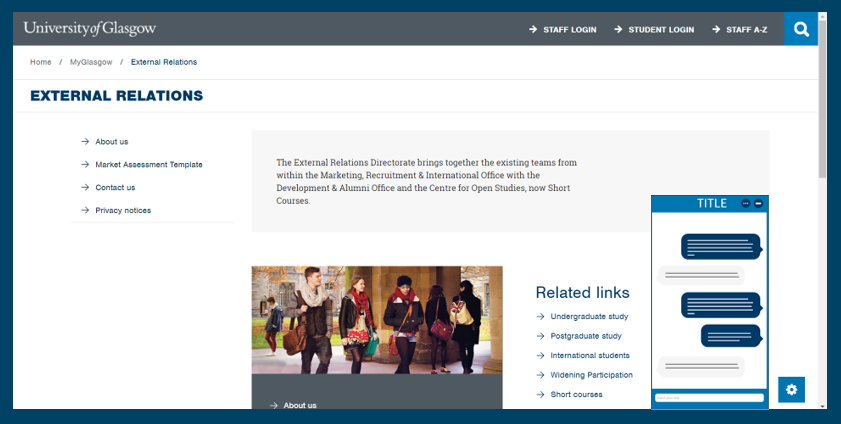
\includegraphics[width=0.85\linewidth]{figures/wireframe-background.png}
    \caption{Initial design mock-up for the chatbot interface}
\end{figure}

\begin{figure}[h!]
    \centering
    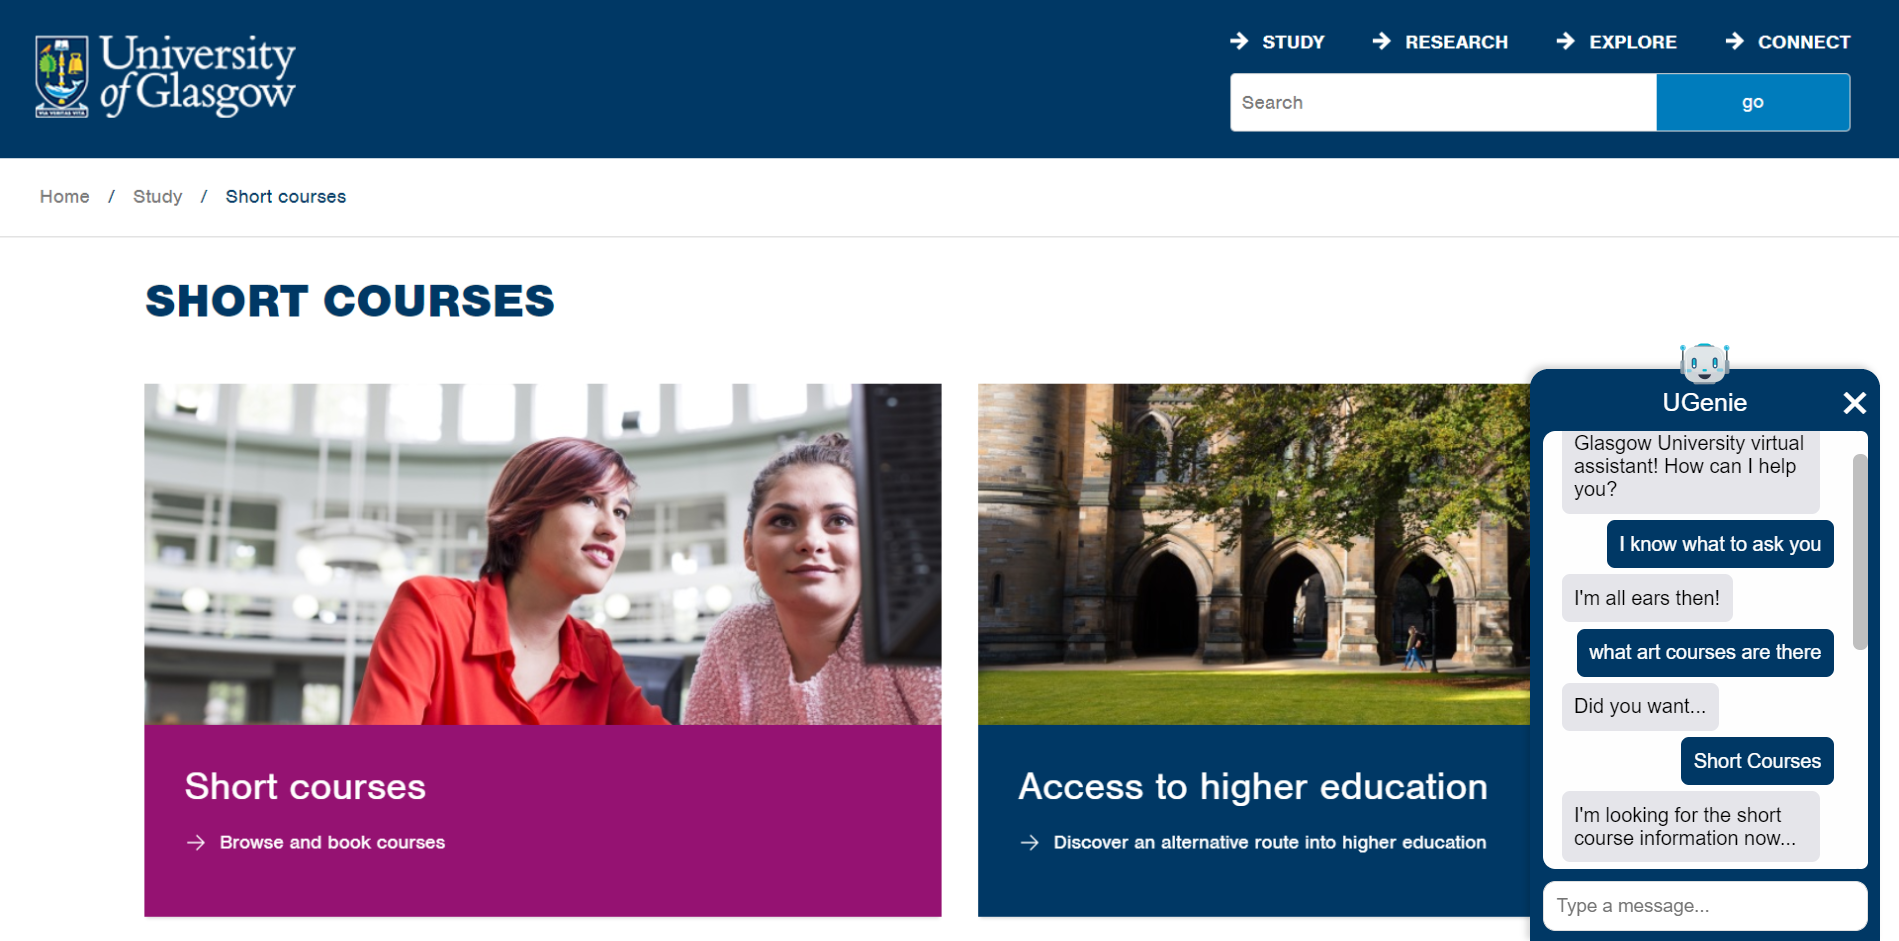
\includegraphics[width=0.85\linewidth]{figures/final-image.PNG}
    \caption{Final interface design as available online}
\end{figure}

\section{MoSCoW User Stories Selection}
\label{apdx:moscow}

\textbf{Must Have:}
\begin{itemize}
\item As an applicant, I want to be able to obtain different kinds of information about the course, such as admission dates and costs, so that I can plan my application.
\item As a potential applicant, I want to have the option to talk to a human instead of a chatbot, so that I can get answers that the chatbot cannot provide.
\end{itemize}

\textbf{Should Have:}
\begin{itemize}
\item As an External Relations employee, I want the bot to have an appropriate tone, so that it conforms to the University\textsc{\char13}s brand guidelines.
\item As a potential applicant, I want to be redirected to more extensive resources if the bot can\textsc{\char13}t give me a satisfying answer, so I can finish my research.
\end{itemize}

\textbf{Could Have:}
\begin{itemize}
\item As a potential applicant, I want to be able to make enquiries on Facebook, so I don\textsc{\char13}t have to look for the chatbot on the University of Glasgow website.
\end{itemize}

\textbf{Would Like to Have:}
\begin{itemize}
\item As a current student, I want to know if the course/short-course I\textsc{\char13}m interested in clashes with anything I currently do, so I know whether I can apply for it.
\end{itemize}

\smallskip
%% for some reason removing small skip puts the figures before Test Coverage
\section{Test Coverage}
\label{apdx:coverage}

\begin{figure}[h]
    \centering
    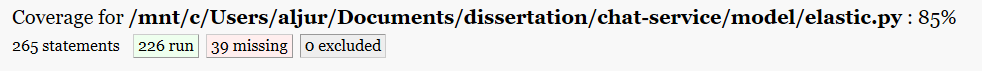
\includegraphics[width=0.85\linewidth]{figures/Unit_Testing_1.PNG}
    \caption{Code coverage of the Python elastic module}
\end{figure}

\begin{figure}[h]
  \centering
  \begin{subfigure}[b]{0.425\linewidth}
    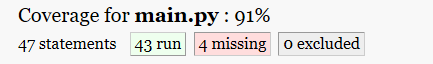
\includegraphics[width=\linewidth]{figures/Unit_Testing_2.PNG}
  \end{subfigure}
  \begin{subfigure}[b]{0.425\linewidth}
    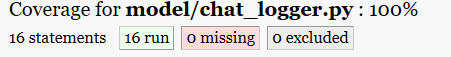
\includegraphics[width=\linewidth]{figures/Unit_Testing_3.PNG}
  \end{subfigure}
  \caption{Code coverage of the Python main and logger modules}
\end{figure}

\section{Planning Poker Estimates in Final Iteration}
\label{apdx:pp}

\begin{figure}[h!]
    \centering
    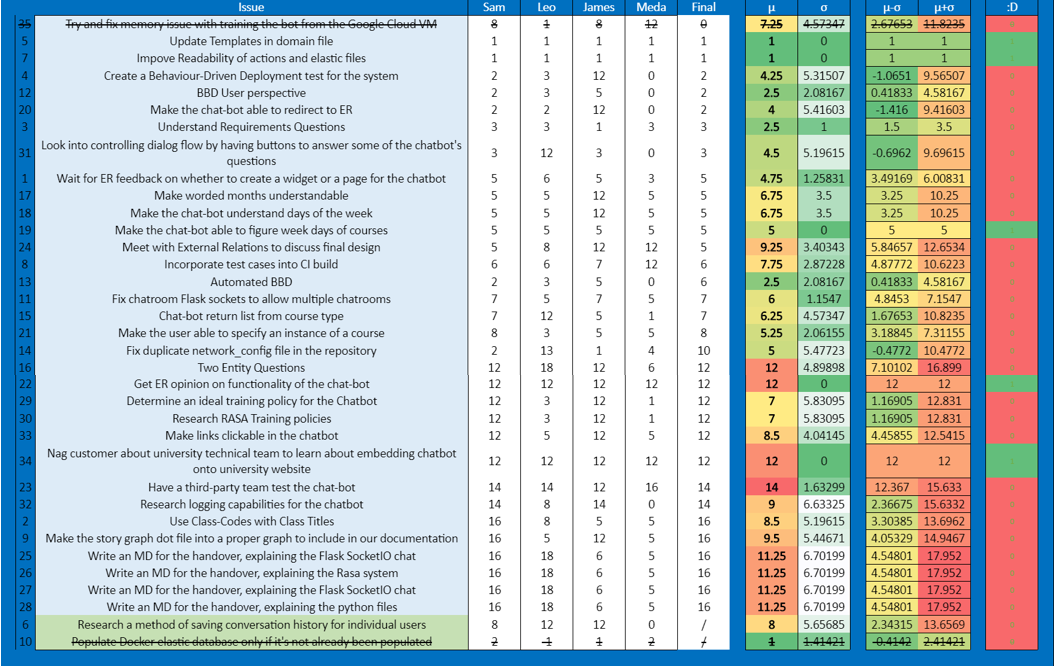
\includegraphics[width=0.85\linewidth]{figures/ppiteration6.PNG}
    \caption{Formatted Excel sheet with our Planning Poker estimations. Metadata includes estimated days, final estimation, average, standard deviation and agreement.}
\end{figure}

\end{document}
